\chapter{Fundamentação Teórica}

\section{Subestações de Energia}
\label{sec:subestacao}

As subestações desempenham um papel crucial na transmissão e distribuição de energia elétrica. Quando a eletricidade é gerada em uma usina, ela é produzida em uma tensão muito alta para minimizar perdas durante a transmissão por longas distâncias. As subestações recebem essa eletricidade de alta tensão e a transformam em níveis de tensão adequados para distribuição aos consumidores finais. Nesse processo, diversos equipamentos são necessários. Nele, existem os transformadores, que são os principais equipamentos responsáveis por essa transformação. Eles elevam a tensão da eletricidade recebida das usinas para tornar a transmissão mais eficiente, reduzindo as perdas de energia no processo. Em seguida, essa eletricidade passa por disjuntores, que protegem o sistema contra sobrecargas e curtos-circuitos, interrompendo o fluxo de corrente elétrica em caso de emergência. Além disso, as subestações também contam com chaves seccionadoras, que permitem isolar partes do sistema elétrico para manutenção ou reparo sem interromper o fornecimento de energia para outras áreas. Os relés de proteção monitoram constantemente o sistema elétrico em busca de falhas e anomalias, acionando os dispositivos de proteção quando necessário para evitar danos aos equipamentos ou interrupções no fornecimento de energia. Os capacitores são usados para corrigir o fator de potência e melhorar a eficiência do sistema, enquanto os reatores de núcleo de ar ajudam a controlar o fluxo de energia e estabilizar a tensão. Todos esses componentes trabalham juntos para garantir que a eletricidade seja transmitida e distribuída de forma segura, confiável e eficiente, atendendo às demandas dos consumidores finais e contribuindo para o funcionamento adequado do sistema elétrico como um todo. Existem também os reatores de núcleo de ar, eles são utilizados principalmente em sistemas de alta tensão para controlar correntes de curto-circuito e proteger equipamentos sensíveis \cite{sen2021principles}.
%Esse livro explica os fundamentos do funcionamento dos equipamentos da geração de energia


\section{Redes Neurais}
\label{sec:redesneurais}

As redes neurais artificiais são modelos computacionais inspirados no funcionamento do cérebro humano, compostos por neurônios interconectados que processam informações. Elas são amplamente utilizadas em diversas áreas, como reconhecimento de padrões, processamento de linguagem natural, visão computacional e muitas outras aplicações de aprendizado de máquina. Em \citeonline{rumelhart1986learning}, descreve-se pioneiramente o algoritmo de retropropagação, fundamental para o treinamento de redes neurais profundas.

Sua estrutura é composta por unidades básicas chamadas de neurônios ou nós, que são organizados em camadas interconectadas. Existem três tipos principais de camadas em uma rede neural: camada de entrada, camadas ocultas e camada de saída.

\begin{itemize}
\item Camada de Entrada: Esta é a camada que recebe os dados de entrada. Cada nó nesta camada representa uma característica ou atributo dos dados que estão sendo alimentados na rede neural. Por exemplo, em uma aplicação de reconhecimento de imagens, cada nó na camada de entrada pode representar um pixel da imagem.
\item Camadas Ocultas: Estas são as camadas intermediárias entre a camada de entrada e a camada de saída. Cada neurônio em uma camada oculta recebe entradas das camadas anteriores, realiza algum tipo de transformação não linear dessas entradas e passa o resultado para a próxima camada. A presença de múltiplas camadas ocultas permite que a rede aprenda representações complexas e abstratas dos dados.
\item Camada de Saída: Esta é a camada final da rede neural que gera as saídas desejadas. A estrutura da camada de saída depende do tipo de problema que está sendo resolvido. Por exemplo, em um problema de classificação, cada nó na camada de saída pode representar uma classe diferente, e a saída pode ser interpretada como a probabilidade de pertencer a cada classe.
\end{itemize}

O funcionamento básico de uma rede neural ocorre em duas fases principais: propagação para a frente (forward propagation) e retropropagação do erro (backpropagation).

\begin{itemize}
\item Propagação para a Frente: Durante esta fase, os dados são alimentados na rede neural através da camada de entrada e propagam-se através das camadas ocultas até a camada de saída. Cada neurônio em cada camada aplica uma transformação às suas entradas e passa o resultado para os neurônios na próxima camada.
\item Retropropagação do Erro: Após a propagação para a frente, a rede compara as saídas previstas com as saídas reais desejadas e calcula a diferença entre elas, chamada de erro. Em seguida, esse erro é propagado de volta através da rede, começando pela camada de saída e indo em direção à camada de entrada. Durante essa retropropagação, os pesos das conexões entre os neurônios são ajustados de acordo com o gradiente do erro em relação aos pesos, usando um algoritmo de otimização como o gradiente descendente, a fim de minimizar o erro global da rede.
\end{itemize}

Essencialmente, as redes neurais aprendem iterativamente ajustando os pesos de suas conexões através do processo de treinamento, onde são apresentados a um conjunto de dados de entrada e as correspondentes saídas desejadas. Com o tempo, a rede neural é capaz de aprender a mapear efetivamente os padrões nos dados de entrada para as saídas desejadas, tornando-se assim capaz de realizar tarefas como reconhecimento de padrões, classificação, regressão, entre outros.

\subsection{You Look Only Once}
\label{sec:yolo}

YOLO (You Only Look Once) é um modelo de detecção de objetos em imagens e vídeos em tempo real, que se destaca por sua eficiência e precisão. Desenvolvido por Joseph Redmon, Santosh Divvala, Ross Girshick e Ali Farhadi, o YOLO aborda o problema de detecção de objetos como uma única tarefa de regressão, prevendo caixas delimitadoras e probabilidades de classe diretamente de imagens inteiras em uma única passagem pela rede neural. O funcionamento do YOLO começa com a divisão da imagem de entrada em uma grade, geralmente de dimensões como 7x7 ou 9x9. Cada célula dessa grade é responsável por prever um conjunto de caixas delimitadoras e as probabilidades das classes dos objetos contidos nessa célula. Para cada célula da grade, o modelo faz previsões sobre as caixas delimitadoras que contêm objetos, representadas por cinco valores: coordenadas (x, y) do centro da caixa, largura (w) e altura (h) da caixa, e a confiança de que a caixa contém um objeto. Além disso, são previstas as probabilidades de cada classe para cada caixa delimitadora. Após a predição das caixas delimitadoras, o YOLO utiliza um processo chamado Non-max Suppression (Supressão de Não-Máximo) para refinar as previsões e eliminar caixas sobrepostas ou redundantes, mantendo apenas as detecções mais confiáveis. Esse processo envolve a supressão de caixas que têm uma sobreposição significativa e a escolha da caixa com a maior confiança entre as caixas sobrepostas. A saída do YOLO é uma lista de caixas delimitadoras, cada uma associada a uma classe prevista e sua confiança. Essas caixas delimitadoras representam os objetos detectados na imagem, fornecendo informações sobre sua localização e classificação. Em resumo, o YOLO oferece uma abordagem eficaz e eficiente para a detecção de objetos em tempo real, consolidando-se como uma ferramenta valiosa em diversas aplicações, desde sistemas de segurança até veículos autônomos \cite{redmon2016youlookonce}.


\subsection{Batch}
\label{sec:batch}

Um dos aspectos cruciais do funcionamento da YOLO é o conceito de "batch" (em tradução livre, "lote") durante o treinamento da rede neural. Ao agrupar várias imagens em lotes para processamento simultâneo, a YOLO aproveita a capacidade de processamento paralelo das GPUs, acelerando significativamente o treinamento. Durante a propagação direta, cada imagem no lote é processada pela rede neural para gerar previsões de detecção de objetos. Em seguida, a perda é calculada em relação às anotações verdadeiras, e os pesos da rede são atualizados para minimizar essa perda, usando algoritmos de otimização como o gradiente descendente. Esse processo é repetido para vários lotes de imagens até que a rede convirja para uma solução adequada. Assim, o uso eficiente de lotes na YOLO não apenas acelera o treinamento, mas também contribui para a robustez e eficácia dos modelos de detecção de objetos resultantes. \cite{goodfellow2016deep}

%A reasonable choice of optimization algorithm is SGD with momentum with a decaying learning rate (popular decay schemes that perform better or worse on
%different problems include decaying linearly until reaching a fixed minimum learning
%rate, decaying exponentially, or decreasing the learning rate by a factor of 2-10
%each time validation error plateaus). Another very reasonable alternative is Adam.
%Batch normalization can have a dramatic effect on optimization performance,
%especially for convolutional networks and networks with sigmoidal nonlinearities.
%While it is reasonable to omit batch normalization from the very first baseline, it
%should be introduced quickly if optimization appears to be problematic.

\subsection{Otimizadores}
\label{sec:otimizadores}

Falar sobre o Otimizadores....!!!

\subsection{Precisão e Recall}
\label{sec:precisaorecall}

A fim de avaliar o desempenho de um treinamento na arquitetura YOLO, é preciso entender os resultados fornecidos pelo modelo. De acordo com \cite{padilla2020survey}, basicamente a YOLO utiliza a métrica chamada Average Precision (AP) (“Precisão Média”, em tradução livre). Ela se baseia no conceito de IoU (“Intersection over the Union”, Intersecção sobre a União, em tradução livre), que calcula uma razão entre a interseção da detecção feita pelo algoritmo com relação à marcação (bounding box) realizada em cima da área dividida pela união dessas duas áreas (Figura 1). Essa razão poderá ser comparada com um valor pré-estabelecido, o thresholds, que será referido por L. A partir desse valor, é possível que no processo de detecção retorne três diferentes resultados na pesquisa pela classe desejada. São eles: Verdadeiro Positivo (VP), Falso Positivo (FP) e Falso Negativo (FN). VP trata-se dos resultados considerados corretos que a rede neural retorna, que seriam todos resultados que IoU > L. FP já seriam os resultados em que IoU < L, que são tidos como incorretos.FN, por sua vez, trata dos resultados totalmente fora do esperado.

\begin{equation}
    \text{Recall} = \frac{VP}{VP + FN} \tag{1}
\end{equation}
    
\begin{equation}
    \text{Precisão} = \frac{VP}{VP + FP} \tag{2}
\end{equation}

Com esses valores, pode-se calcular os resultados da saída que o treinamento da rede YOLO fornece. Em (1), tem-se o cálculo da Recall, que calcula a capacidade da rede de detectar todos os objetos relevantes em uma imagem. Já a Precisão (2), refere-se à capacidade da rede de encontrar apenas resultados relevantes. 

\begin{figure}[!h]
    \center
    \begin{minipage}{0.6\linewidth}
    \center
    \captionsetup{justification=centering,margin=0.5cm,font=small}
    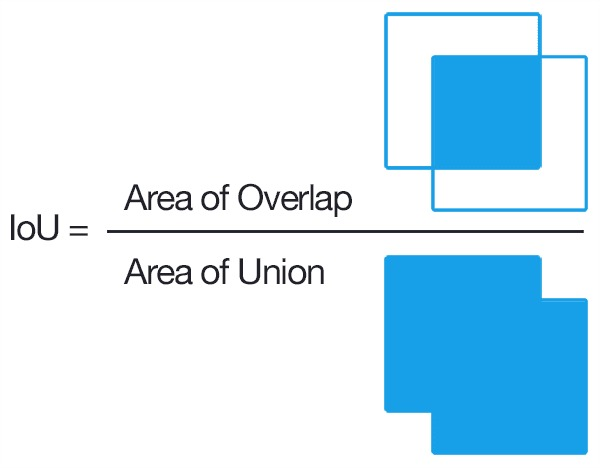
\includegraphics[width=0.7\linewidth]{img/cap2/iou.png}
    \caption{ Cálculo de IoU. \cite{padilla2020survey}} \label{subfig:iou}
    \end{minipage}
\end{figure}

A arquitetura YOLO disponibiliza um dataset, ou seja, um banco de imagens e weights, comum em todas as versões, chamado de COCO (“Common Objects in Context”, que em tradução livre seria “Classes Comuns de Objetos”) com classes pré-treinadas e imagens para realização de treinamentos. A partir dele, verificou-se por meio de testes a eficiência das quatro últimas versões da YOLO, a fim de identificar se nas mais recentes houve melhoras significativas em termos de performance e precisão. Na Figura 1, é apresentado o comparativo das versões. Nota-se que a v8, para um menor número de parâmetros que as demais, apresentou uma mAP50-95, maior que nas versões v5, v6 e v7. Além disso, com relação a velocidade de processamento, a v8 também se sobressai, com maior rapidez no processamento, ao processar maior quantidade de imagens para um mesmo intervalo de tempo \cite{padilla2020survey}.

\begin{figure}[!h]
    \center
    \begin{minipage}{0.9\linewidth}
    \center
    \captionsetup{justification=centering,margin=0.5cm,font=small}
    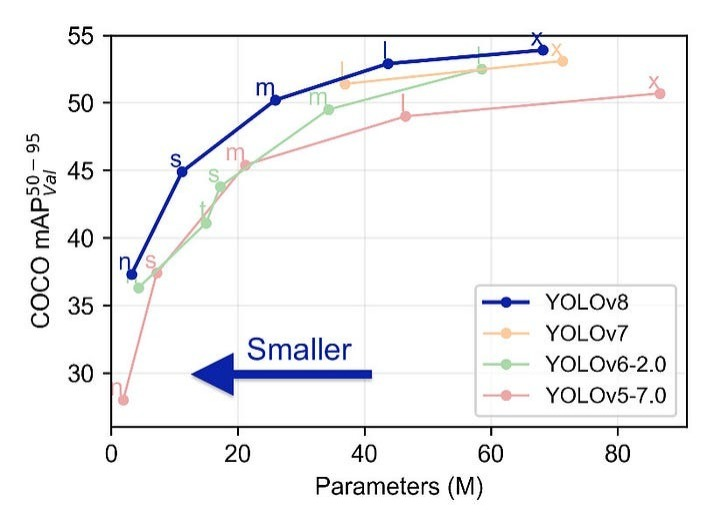
\includegraphics[width=0.7\linewidth]{img/cap2/precisao.png}
    \caption{ Aumento de desempenho da precisão média, versão 5 para 8.  \cite{ultralytics2023yolo}} \label{subfig:precisao}
    \end{minipage}
\end{figure}

\section{Realidade Virtual}
\label{sec:precisaorecall}

A realidade virtual é uma tecnologia que permite aos usuários imergirem em ambientes virtuais tridimensionais, geralmente através do uso de dispositivos como óculos de realidade virtual (VR) ou capacetes. Desde suas primeiras manifestações nas décadas de 1960 e 1970, quando ainda era experimental e limitada, a realidade virtual tem evoluído consideravelmente. No entanto, foi na década de 1990 que essa tecnologia começou a ganhar destaque comercial, com o lançamento de dispositivos como o Virtual Boy da Nintendo e os primeiros sistemas de realidade virtual para computadores pessoais. Desde então, a realidade virtual tem sido aplicada em uma variedade de campos, incluindo jogos, simulações, treinamento, educação e terapia. Sua popularidade continuou a crescer com o avanço da tecnologia, oferecendo experiências cada vez mais imersivas e acessíveis \cite{kirner2011evoluccao}.

%Citar trabalho alexandre
%O artigo de kirner2011evoluccao, faz um panorama da história da realidade virtual.

\section{Considerações finais}

Neste capítulo, foi apresentado o arcabouço teórico necessário para o entendimento da proposta dessa dissertação. A apresentação das redes neurais, e em específico, o modo que a arquitetura da YOLOv8 sobrepõe-se em termos de eficiência em relação às demais arquiteturas abordadas em outros trabalhos científicos, demonstra o direcionamento assertivo deste trabalho. Além disso, a apresentação da Realidade Virtual como uma disciplina inovadora e muito útil para servir à diversos propósitos dentro da indústria e ciência, corroboram para o entendimento da proposta desta dissertação.